\chapter{Nonlinear Transformation}
\lecture{12}{21 Oct.}{}

\begin{prev}
    Linear classification, linear regression and logistic regression now cover
    binary, soft, real-valued and multiclass outputs, all with efficient
    algorithms. Every one of them decides by the score \(s = \bm{w}^\top
    \bm{x}\), so every boundary they can draw is a hyperplane in the original
    \(\bm{x}\)-space.
\end{prev}

This chapter removes that restriction without writing a single new algorithm.
\begin{enumerate}
    \item A circle in \(\mathcal{X}\) turns out to be a line in a transformed
        space \(\mathcal{Z}\).
    \item Hence any linear model run on transformed data gives a nonlinear model
        on the original data.
    \item The transform has a price, in computation and in VC dimension.
    \item Polynomial transforms nest into a chain of hypothesis sets, which
        tells us where to start: with the linear model.
\end{enumerate}

\section{Quadratic Hypotheses}\label{sec:quad-hyp}

\source{slides p.2--7}

\subsection{Linear Hypotheses}

Up to now: linear hypotheses. But limited \ldots

\begin{center}
    \begin{tikzpicture}[scale=1.3]
        \fill[neghalf] (-1,-1) -- (0.4,-1) -- (0,1) -- (-1,1) -- cycle;
        \fill[poshalf] (0.4,-1) -- (1,-1) -- (1,1) -- (0,1) -- cycle;
        \draw[sepline] (0.4,-1) -- (0,1);
        \foreach \p in {(0.35,0.6), (0.39,0.0), (0.43,-0.6), (0.8,-0.3),
            (0.9,0.3)}{\node[dpos] at \p {};}
        \foreach \p in {(-0.6,0.7), (-0.3,-0.35), (-0.1,0.5), (0.1,-0.8)}
            {\node[dneg] at \p {\(\times\)};}
        \draw[plotbox] (-1,-1) rectangle (1,1);
    \end{tikzpicture}
    \hspace{1.6cm}
    \begin{tikzpicture}[scale=1.3]
        \circdataX
        \xplotframe
    \end{tikzpicture}
\end{center}

\begin{itemize}
    \item visually: `line'-like boundary;
    \item mathematically: linear scores \(s = \bm{w}^\top \bm{x}\);
    \item theoretically: \(\dvc\) under control :-);
    \item practically: on some \(\mathcal{D}\), large \(\Ein\) for every line
        :-(.
\end{itemize}

The first two are the definition of the perceptron (\autoref{def:perceptron}),
the third is \autoref{thm:vc-perceptron}: \(\dvc = d + 1\), so a modest \(N\)
already makes \(\Ein \approx \Eout\). The fourth is the right-hand data set,
which will be with us for the whole chapter.

\begin{observation}
    No line separates the right-hand data. The four crosses nearest the corners
    span a quadrilateral containing the circle at \((0.002, 0.138)\), so that
    circle is a convex combination \(\sum_i \lambda_i \bm{x}_i\) of crosses. Any
    \(\bm{w}\) with negative score on every cross then has \(\bm{w}^\top
    (1, \sum_i \lambda_i \bm{x}_i) = \sum_i \lambda_i \bm{w}^\top (1, \bm{x}_i)
    < 0\) on the circle too.
\end{observation}

\begin{question}
    How to \textbf{break the limit} of linear hypotheses?
\end{question}

\subsection{Circular Separable}

\begin{center}
    \begin{tikzpicture}[scale=1.3]
        \circdataX
        \xplotframe
    \end{tikzpicture}
    \hspace{1.6cm}
    \begin{tikzpicture}[scale=1.3]
        \fill[neghalf] (-1,-1) rectangle (1,1);
        \fill[poshalf] (0,0) circle ({sqrt(0.6)});
        \draw[sepline] (0,0) circle ({sqrt(0.6)});
        \circdataX
        \xplotframe
    \end{tikzpicture}
\end{center}

\begin{itemize}
    \item \(\mathcal{D}\) not linear separable;
    \item but \textbf{circular separable} by a circle of radius \(\sqrt{0.6}\)
        centered at origin:
        \[
            h_{\mathrm{SEP}}(\bm{x}) = \sign \left( -x_1^2 - x_2^2 + 0.6
            \right) .
        \]
\end{itemize}

\(h_{\mathrm{SEP}}\) says \(+1\) exactly inside the circle \(x_1^2 + x_2^2 =
0.6\), and the data agree with it on every example.

\begin{question}
    Re-derive \textbf{Circular}-PLA, \textbf{Circular}-Regression, blahblah
    \ldots\ all over again? :-)
\end{question}

\subsection{Circular Separable and Linear Separable}

Read \(h_{\mathrm{SEP}}\) term by term, as a weighted sum:
\begin{align*}
    h(\bm{x}) &= \sign \Bigl( \underbrace{0.6}_{\tilde{w}_0} \cdot
    \underbrace{1}_{z_0} + \underbrace{(-1)}_{\tilde{w}_1} \cdot
    \underbrace{x_1^2}_{z_1} + \underbrace{(-1)}_{\tilde{w}_2} \cdot
    \underbrace{x_2^2}_{z_2} \Bigr)\\
    &= \sign \left( \tilde{\bm{w}}^\top \bm{z} \right) .
\end{align*}
The formula is still linear --- in the new variables \(z_1 = x_1^2\), \(z_2 =
x_2^2\) rather than in \(x_1, x_2\).

\begin{center}
    \begin{tikzpicture}
        \begin{scope}[scale=1.3]
            \fill[neghalf] (-1,-1) rectangle (1,1);
            \fill[poshalf] (0,0) circle ({sqrt(0.6)});
            \draw[sepline] (0,0) circle ({sqrt(0.6)});
            \circdataX
            \circlabelsX
            \xplotframe
        \end{scope}
        \draw[mlarrow] (1.75,0) -- (3.45,0) node[midway, above]
            {\(\bm{\Phi}\)};
        \begin{scope}[shift={(4.0,-1.175)}, scale=2.5]
            \fill[neghalf] (-0.05,-0.05) rectangle (1,1);
            \fill[poshalf] (-0.05,-0.05) -- (0.65,-0.05) -- (-0.05,0.65)
                -- cycle;
            \draw[sepline] (0.65,-0.05) -- (-0.05,0.65);
            \circdataZ
            \circlabelsZ
            \zplotframe
        \end{scope}
    \end{tikzpicture}
\end{center}

\begin{itemize}
    \item \(\{(\bm{x}_n, y_n)\}\) circular separable \(\Longrightarrow\)
        \(\{(\bm{z}_n, y_n)\}\) linear separable;
    \item \(\bm{x} \in \mathcal{X} \overset{\bm{\Phi}}{\longmapsto} \bm{z} \in
        \mathcal{Z}\): \textbf{(nonlinear) feature transform \(\bm{\Phi}\)}.
\end{itemize}

\begin{definition}[Feature transform]\label{def:feature-transform}
    A \vocab{feature transform} is a map \(\bm{\Phi} \colon \mathcal{X} \to
    \mathcal{Z}\), \(\bm{z} = \bm{\Phi}(\bm{x})\), whose first coordinate is the
    constant \(z_0 = 1\). \(\mathcal{Z}\) is the \vocab{\(\mathcal{Z}\)-space}
    and \(\bm{z}_n = \bm{\Phi}(\bm{x}_n)\) the transformed examples. Here
    \(\bm{\Phi}(\bm{x}) = (1, x_1^2, x_2^2)\).
\end{definition}

\begin{notation}
    A tilde marks objects living in \(\mathcal{Z}\): weights
    \(\tilde{\bm{w}}\), hypotheses \(\tilde{h}\), and \(\tilde{d}\) for the
    dimension of \(\mathcal{Z}\) not counting \(z_0\). Plain \(z_i\) is a
    coordinate of \(\bm{z}\); bold \(\bm{z}_n\) is the \(n\)-th transformed
    example. In the pictures, \(\bm{x}_1\) (a circle) lands at \(\bm{z}_1\)
    and \(\bm{x}_2\) (a cross) at \(\bm{z}_2\).
\end{notation}

Squaring sends both \(\pm x_i\) to the same \(z_i \ge 0\), so the whole of
\(\mathcal{X}\) folds into the corner \(z_1, z_2 \ge 0\): circles near the
origin of \(\mathcal{X}\) land near the origin of \(\mathcal{Z}\), crosses near
the corners of \(\mathcal{X}\) land far out, and the circle \(x_1^2 + x_2^2 =
0.6\) becomes the line \(z_1 + z_2 = 0.6\).

\begin{question}
    Circular separable in \(\mathcal{X}\) \(\Longrightarrow\) linear separable
    in \(\mathcal{Z}\); vice versa?
\end{question}

Not quite. A line in \(\mathcal{Z}\) pulls back to \(\tilde{w}_0 + \tilde{w}_1
x_1^2 + \tilde{w}_2 x_2^2 = 0\), which is a circle only for special weights ---
the next subsection lists what else it can be.

\subsection{Linear Hypotheses in \texorpdfstring{\(\mathcal{Z}\)}{Z}-Space}

\[
    (z_0, z_1, z_2) = \bm{z} = \bm{\Phi}(\bm{x}) = (1, x_1^2, x_2^2),
\]
\[
    h(\bm{x}) = \tilde{h}(\bm{z}) = \sign \left( \tilde{\bm{w}}^\top
    \bm{\Phi}(\bm{x}) \right) = \sign \left( \tilde{w}_0 + \tilde{w}_1 x_1^2 +
    \tilde{w}_2 x_2^2 \right) .
\]

\(\tilde{\bm{w}} = (\tilde{w}_0, \tilde{w}_1, \tilde{w}_2)\):
\begin{itemize}
    \item \((0.6, -1, -1)\): circle (\(\circ\) inside);
    \item \((-0.6, +1, +1)\): circle (\(\circ\) outside);
    \item \((0.6, -1, -2)\): ellipse;
    \item \((0.6, -1, +2)\): hyperbola;
    \item \((0.6, +1, +2)\): constant \(\circ\) :-).
\end{itemize}

Each case is the sign pattern of \(\tilde{\bm{w}}\).
\begin{itemize}
    \item \textbf{Circles}: \(\tilde{w}_1 = \tilde{w}_2\) with the opposite sign
        to \(\tilde{w}_0\); negating all three keeps the curve and swaps the
        sides, which is why \(\circ\) moves from inside to outside.
    \item \textbf{Ellipse}: unequal weights of the same sign, \(x_1^2 + 2x_2^2 =
        0.6\).
    \item \textbf{Hyperbola}: weights of opposite signs, \(x_1^2 - 2x_2^2 =
        0.6\).
    \item \textbf{Constant}: all positive, so \(0.6 + x_1^2 + 2x_2^2 > 0\) for
        every \(\bm{x}\): there is no boundary at all.
\end{itemize}
What is missing is just as telling: every curve here is centred at the origin,
with axes along \(x_1\) and \(x_2\), because \(\bm{\Phi}\) sees only \(x_1^2\)
and \(x_2^2\) and cannot tell \(x_i\) from \(-x_i\). A circle centred anywhere
else, or a tilted ellipse, is out of reach.

\begin{moral}
    Lines in \(\mathcal{Z}\)-space \(\iff\) \textbf{special} quadratic curves in
    \(\mathcal{X}\)-space.
\end{moral}

\subsection{General Quadratic Hypothesis Set}

The missing curves need the missing terms. A `bigger' \(\mathcal{Z}\)-space
with
\[
    \bm{\Phi}_2(\bm{x}) = (1, x_1, x_2, x_1^2, x_1 x_2, x_2^2)
\]
keeps all monomials of degree at most \(2\): perceptrons in
\(\mathcal{Z}\)-space \(\iff\) quadratic hypotheses in \(\mathcal{X}\)-space.

\begin{definition}[Quadratic hypothesis set]\label{def:quad-hyp-set}
    \[
        \mathcal{H}_{\bm{\Phi}_2} = \left\{ h(\bm{x}) : h(\bm{x}) = \tilde{h}
        \left( \bm{\Phi}_2(\bm{x}) \right) \text{ for some linear } \tilde{h}
        \text{ on } \mathcal{Z} \right\} .
    \]
\end{definition}

\begin{itemize}
    \item can implement \textbf{all possible quadratic curve boundaries}:
        circle, ellipse, \textbf{rotated} ellipse, hyperbola, parabola,
        \ldots
        \[
            \text{ellipse } 2(x_1 + x_2 - 3)^2 + (x_1 - x_2 - 4)^2 = 1
            \quad \Longleftarrow \quad \tilde{\bm{w}}^\top = [33, -20, -4, 3,
            2, 3] ;
        \]
    \item include \textbf{lines and constants as degenerate cases}.
\end{itemize}

\begin{eg}[The rotated ellipse]
    Expanding,
    \begin{align*}
        2(x_1 + x_2 - 3)^2 &= 2x_1^2 + 4x_1 x_2 + 2x_2^2 - 12x_1 - 12x_2 + 18,\\
        (x_1 - x_2 - 4)^2 &= x_1^2 - 2x_1 x_2 + x_2^2 - 8x_1 + 8x_2 + 16,
    \end{align*}
    so the ellipse is \(33 - 20x_1 - 4x_2 + 3x_1^2 + 2x_1 x_2 + 3x_2^2 = 0\),
    whose coefficients in the order of \(\bm{\Phi}_2\) are exactly
    \(\tilde{\bm{w}}\). The cross term \(2x_1 x_2\) tilts the axes, and the
    linear terms move the centre to \((3.5, -0.5)\), where \(x_1 + x_2 = 3\)
    and \(x_1 - x_2 = 4\). Far from the centre the quadratic part dominates and
    is positive, so this \(\tilde{\bm{w}}\) says \(\circ\) outside the ellipse.
\end{eg}

Setting \(\tilde{w}_3 = \tilde{w}_4 = \tilde{w}_5 = 0\) leaves \(\sign(\tilde{w}_0
+ \tilde{w}_1 x_1 + \tilde{w}_2 x_2)\), an ordinary perceptron; zeroing all but
\(\tilde{w}_0\) leaves a constant. So the perceptrons sit inside
\(\mathcal{H}_{\bm{\Phi}_2}\) --- the quadratic set only adds options.

\begin{moral}
    Next: \textbf{learn} a good quadratic hypothesis \(g\).
\end{moral}

\begin{exercise}[Fun Time]
    Using the transform \(\bm{\Phi}_2(\bm{x}) = (1, x_1, x_2, x_1^2, x_1 x_2,
    x_2^2)\), which of the following weights \(\tilde{\bm{w}}^\top\) in the
    \(\mathcal{Z}\)-space implements the parabola \(2x_1^2 + x_2 = 1\)?
    \begin{enumerate}[(1)]
        \item \([-1, 2, 1, 0, 0, 0]\);
        \item \([0, 2, 1, 0, -1, 0]\);
        \item \([-1, 0, 1, 2, 0, 0]\);
        \item \([-1, 2, 0, 0, 0, 1]\).
    \end{enumerate}
\end{exercise}

\begin{proof}[Reference Answer]
    (3). Too simple, uh? :-) Flexibility to implement arbitrary quadratic
    curves opens new possibilities for minimizing \(\Ein\)! Indeed \(2x_1^2 +
    x_2 = 1\) is \(-1 + 0 \cdot x_1 + 1 \cdot x_2 + 2 x_1^2 + 0 \cdot x_1 x_2 +
    0 \cdot x_2^2 = 0\). The others are the line \(2x_1 + x_2 = 1\), the
    hyperbola \(2x_1 + x_2 = x_1 x_2\), and the sideways parabola \(2x_1 +
    x_2^2 = 1\).
\end{proof}

\section{Nonlinear Transform}\label{sec:nonlin-transform}

\source{slides p.8--12}

\(\mathcal{H}_{\bm{\Phi}_2}\) is defined through perceptrons on
\(\mathcal{Z}\); what is still missing is a way to \emph{learn} in it.

\subsection{Good Quadratic Hypothesis}

\begin{center}
    \begin{tabular}{@{}ccc@{}}
        \(\mathcal{Z}\)-space & & \(\mathcal{X}\)-space\\
        perceptrons & \(\iff\) & quadratic hypotheses\\
        \textbf{good perceptron} & \(\iff\) & \textbf{good quadratic
        hypothesis}\\
        \textbf{separating perceptron} & \(\iff\) & \textbf{separating
        quadratic hypothesis}
    \end{tabular}
\end{center}

\begin{center}
    \begin{tikzpicture}
        \begin{scope}[shift={(-1.175,-1.175)}, scale=2.5]
            \fill[neghalf] (-0.05,-0.05) rectangle (1,1);
            \fill[poshalf] (-0.05,-0.05) -- (0.65,-0.05) -- (-0.05,0.65)
                -- cycle;
            \draw[sepline] (0.65,-0.05) -- (-0.05,0.65);
            \circdataZ
            \circlabelsZ
            \zplotframe
        \end{scope}
        \node at (2.8,0) {\(\iff\)};
        \begin{scope}[shift={(5.3,0)}, scale=1.3]
            \fill[neghalf] (-1,-1) rectangle (1,1);
            \fill[poshalf] (0,0) circle ({sqrt(0.6)});
            \draw[sepline] (0,0) circle ({sqrt(0.6)});
            \circdataX
            \circlabelsX
            \xplotframe
        \end{scope}
    \end{tikzpicture}
\end{center}

\begin{itemize}
    \item want: get \textbf{good perceptron} in \(\mathcal{Z}\)-space;
    \item known: get \textbf{good perceptron} in \(\mathcal{X}\)-space with data
        \(\{(\bm{x}_n, y_n)\}\).
\end{itemize}

The two rows of `\(\iff\)' are one identity, applied example by example:

\begin{lemma}[Same in-sample error after the transform]\label{lem:same-ein-z}
    Let \(h(\bm{x}) = \tilde{h}(\bm{\Phi}(\bm{x}))\). Then \(h\) on
    \(\{(\bm{x}_n, y_n)\}\) and \(\tilde{h}\) on \(\{(\bm{z}_n, y_n)\}\) make
    mistakes on exactly the same \(n\), so their \(\Ein\) are equal.
\end{lemma}

\begin{proof}
    \(h(\bm{x}_n) = \tilde{h}(\bm{\Phi}(\bm{x}_n)) = \tilde{h}(\bm{z}_n)\), and
    the label \(y_n\) is the same in both data sets.
\end{proof}

So a good (or separating) perceptron for the transformed data \emph{is} a good
(or separating) quadratic hypothesis for the original data, and the algorithm
needs no change --- only its input does.

\begin{moral}
    Todo: get \textbf{good perceptron} in \(\mathcal{Z}\)-space with data
    \(\{(\bm{z}_n = \bm{\Phi}_2(\bm{x}_n), y_n)\}\).
\end{moral}

\subsection{The Nonlinear Transform Steps}

\begin{center}
    \begin{tikzpicture}
        \begin{scope}[scale=1.1]
            \circdataX
            \xplotframe
        \end{scope}
        \draw[mlarrow] (1.4,0) -- (3.2,0) node[midway, above]
            {\(\bm{\Phi}\)};
        \begin{scope}[shift={(3.705,-0.995)}, scale=2.1]
            \circdataZ
            \zplotframe
        \end{scope}
        \draw[mlarrow] (4.8,-1.45) -- (4.8,-2.0) node[midway, right]
            {\(\mathcal{A}\)};
        \begin{scope}[shift={(0,-3.4)}, scale=1.1]
            \fill[neghalf] (-1,-1) rectangle (1,1);
            \fill[poshalf] (0,0) ellipse ({1} and {sqrt(0.6)});
            \draw[sepline] (0,0) ellipse ({1} and {sqrt(0.6)});
            \circdataX
            \xplotframe
        \end{scope}
        \draw[mlarrow, draw=black!30] (3.2,-3.15) -- (1.4,-3.15)
            node[midway, above, text=black!40] {\(\bm{\Phi}^{-1}\)};
        \draw[mlarrow] (1.4,-3.65) -- (3.2,-3.65) node[midway, above]
            {\(\bm{\Phi}\)};
        \begin{scope}[shift={(3.705,-4.395)}, scale=2.1]
            \fill[neghalf] (-0.05,-0.05) rectangle (1,1);
            \fill[poshalf] (-0.05,-0.05) -- (1,-0.05) -- (1,0) -- (-0.05,0.63)
                -- cycle;
            \draw[sepline] (1,0) -- (-0.05,0.63);
            \circdataZ
            \zplotframe
        \end{scope}
    \end{tikzpicture}
\end{center}

\begin{algorithm}[H]
    \caption{Learning with a Feature Transform}\label{alg:feature-transform}
    \KwIn{training examples \(\mathcal{D} = \{(\bm{x}_n, y_n)\}\), a feature
    transform \(\bm{\Phi}\), a linear classification algorithm \(\mathcal{A}\)}
    \KwOut{the hypothesis \(g\)}
    transform original data \(\{(\bm{x}_n, y_n)\}\) to \(\{(\bm{z}_n =
    \bm{\Phi}(\bm{x}_n), y_n)\}\) by \(\bm{\Phi}\)\;
    get a good perceptron \(\tilde{\bm{w}}\) using \(\{(\bm{z}_n, y_n)\}\) and
    your favorite linear classification algorithm \(\mathcal{A}\)\;
    \Return \(g(\bm{x}) = \sign \left( \tilde{\bm{w}}^\top \bm{\Phi}(\bm{x})
    \right)\)\;
\end{algorithm}

Two things in the picture deserve a second look.
\begin{itemize}
    \item \textbf{An ellipse, not the circle}: the line \(\mathcal{A}\)
        returned (bottom right) is \(0.6 z_1 + z_2 = 0.6\), i.e.\
        \(\tilde{\bm{w}} = (0.6, -0.6, -1)\), not the \((0.6, -1, -1)\) we
        designed by hand. It separates the transformed data just as well, and
        back in \(\mathcal{X}\) it is the ellipse \(x_1^2 + x_2^2/0.6 = 1\).
        By \autoref{lem:same-ein-z} both have \(\Ein = 0\); \(\mathcal{A}\) has
        no reason to prefer the circle.
    \item \textbf{The grey \(\bm{\Phi}^{-1}\)}: \(\bm{\Phi}\) is not
        invertible --- \(\bm{x}\) and \(-\bm{x}\) have the same \(\bm{z}\) ---
        and the algorithm never inverts it. Step 3 carries the boundary back
        by \emph{composing} with \(\bm{\Phi}\): \(g\) says \(\circ\) on the
        set of \(\bm{x}\) whose image lies on the \(\circ\) side of the line.
        The arrow is only a picture of that preimage.
\end{itemize}

\subsection{Nonlinear Model via Nonlinear \texorpdfstring{\(\bm{\Phi}\)}{Phi}
+ Linear Models}

\begin{center}
    \begin{minipage}[c]{0.56\textwidth}
        \centering
        \begin{tikzpicture}[scale=0.72]
            \begin{scope}[scale=1.1]
                \circdataX
                \draw[plotbox] (-1,-1) rectangle (1,1);
            \end{scope}
            \draw[mlarrow] (1.4,0) -- (3.2,0) node[midway, above]
                {\(\bm{\Phi}\)};
            \begin{scope}[shift={(3.705,-0.995)}, scale=2.1]
                \circdataZ
                \draw[plotbox] (-0.05,-0.05) rectangle (1,1);
            \end{scope}
            \draw[mlarrow] (4.8,-1.25) -- (4.8,-2.0) node[midway, right]
                {\(\mathcal{A}\)};
            \begin{scope}[shift={(0,-3.4)}, scale=1.1]
                \fill[neghalf] (-1,-1) rectangle (1,1);
                \fill[poshalf] (0,0) ellipse ({1} and {sqrt(0.6)});
                \draw[sepline] (0,0) ellipse ({1} and {sqrt(0.6)});
                \circdataX
                \draw[plotbox] (-1,-1) rectangle (1,1);
            \end{scope}
            \draw[mlarrow, draw=black!30] (3.2,-3.1) -- (1.4,-3.1)
                node[midway, above, text=black!40] {\(\bm{\Phi}^{-1}\)};
            \draw[mlarrow] (1.4,-3.7) -- (3.2,-3.7) node[midway, above]
                {\(\bm{\Phi}\)};
            \begin{scope}[shift={(3.705,-4.395)}, scale=2.1]
                \fill[neghalf] (-0.05,-0.05) rectangle (1,1);
                \fill[poshalf] (-0.05,-0.05) -- (1,-0.05) -- (1,0)
                    -- (-0.05,0.63) -- cycle;
                \draw[sepline] (1,0) -- (-0.05,0.63);
                \circdataZ
                \draw[plotbox] (-0.05,-0.05) rectangle (1,1);
            \end{scope}
        \end{tikzpicture}
    \end{minipage}%
    \hfill
    \begin{minipage}[c]{0.4\textwidth}
        Two choices:
        \begin{itemize}
            \item feature transform \(\bm{\Phi}\);
            \item linear model \(\mathcal{A}\), \textbf{not just binary
                classification}.
        \end{itemize}
    \end{minipage}
\end{center}

\autoref{alg:feature-transform} never used that \(\mathcal{A}\) is a
classifier: step 2 hands \(\{(\bm{z}_n, y_n)\}\) to \emph{any} linear model of
the previous chapters, and step 3 returns that model's own output applied to
\(\bm{\Phi}(\bm{x})\) --- \(\tilde{\bm{w}}^\top \bm{\Phi}(\bm{x})\) for linear
regression, \(\theta(\tilde{\bm{w}}^\top \bm{\Phi}(\bm{x}))\) for logistic
regression. The two knobs are independent.

\begin{moral}
    Pandora's box :-): can now freely do \textbf{quadratic PLA, quadratic
    regression, cubic regression, \ldots, polynomial regression}.
\end{moral}

\subsection{Feature Transform \texorpdfstring{\(\bm{\Phi}\)}{Phi}}

The same diagram, on the digit data of \autoref{def:raw}: each image is
reduced to two numbers, its average intensity and its symmetry, and the
task is `1' (\(\circ\)) against `not 1' (\(\times\)).

\begin{center}
    \begin{adjustbox}{max width=\textwidth}
        \begin{tikzpicture}
            \node (grid) at (3.35,0)
                {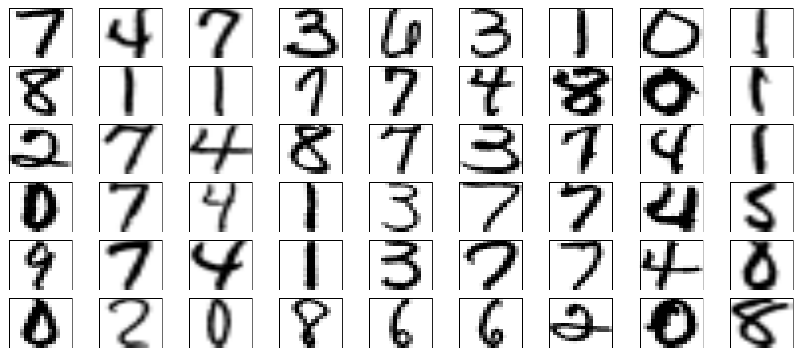
\includegraphics[width=6.7cm]{Figures/digits_grid.png}};
            \node (raw) at (11,0)
                {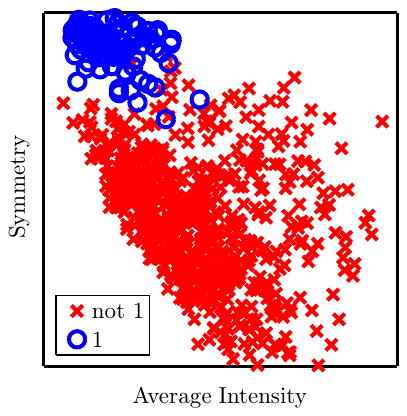
\includegraphics[width=3.6cm]{Figures/one_vs_not_one_data.png}};
            \node (boxed) at (3.35,-4.6)
                {
\includegraphics[width=6.7cm]{Figures/digits_classified.png}};
            \node (fit) at (11,-4.6)
                {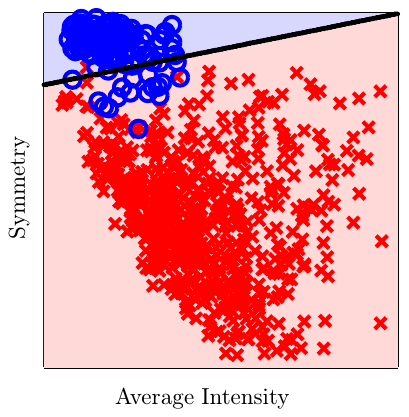
\includegraphics[width=3.6cm]{Figures/one_vs_not_one_fit.png}};
            \draw[mlarrow] (7.15,0) -- (8.95,0) node[midway, above]
                {\(\bm{\Phi}\)};
            \draw[mlarrow] (11,-2.0) -- (11,-2.55) node[midway, right]
                {\(\mathcal{A}\)};
            \draw[mlarrow, draw=black!30] (8.95,-4.3) -- (7.15,-4.3)
                node[midway, above, text=black!40] {\(\bm{\Phi}^{-1}\)};
            \draw[mlarrow] (7.15,-4.9) -- (8.95,-4.9) node[midway, above]
                {\(\bm{\Phi}\)};
        \end{tikzpicture}
    \end{adjustbox}
\end{center}

Top left are raw \(16 \times 16\) images, each a point of \(\mathbb{R}^{256}\);
\(\bm{\Phi}\) computes the two features, after which the `1's (thin, so dark
on few pixels, and symmetric) crowd into the upper left. A linear
classifier in that plane draws one line, and a new image is classified by
computing its features and checking the side: the bottom row shows the result,
a blue frame for `1' and red for `not 1'. As before, \(\bm{\Phi}^{-1}\) is
grey --- two numbers cannot be turned back into an image, and need not be.

\begin{moral}
    Not new, not just polynomial:\\
    \null\hfill raw (pixels) \(\xrightarrow{\text{domain knowledge}}\)
    concrete (intensity, symmetry).\hfill\null
\end{moral}

This is the conversion of \autoref{def:raw} into \autoref{def:concrete}
features, seen in a new light: hand-made features were feature transforms all
along, and a polynomial transform is just one that needs no domain knowledge.

\begin{question}
    The force, too good to be true? :-)
\end{question}

\begin{exercise}[Fun Time]
    Consider the quadratic transform \(\bm{\Phi}_2(\bm{x})\) for \(\bm{x} \in
    \mathbb{R}^d\) instead of in \(\mathbb{R}^2\). The transform should include
    all different quadratic, linear, and constant terms formed by \((x_1, x_2,
    \dots, x_d)\). What is the number of dimensions of \(\bm{z} =
    \bm{\Phi}_2(\bm{x})\)?
    \begin{enumerate}[(1)]
        \item \(d\);
        \item \(\frac{d^2}{2} + \frac{3d}{2} + 1\);
        \item \(d^2 + d + 1\);
        \item \(2^d\).
    \end{enumerate}
\end{exercise}

\begin{proof}[Reference Answer]
    (2). Number of different quadratic terms is \(\binom{d}{2} + d\); number of
    different linear terms is \(d\); number of different constant term is
    \(1\). The quadratic terms are the cross terms \(x_i x_j\), \(i < j\), and
    the squares \(x_i^2\); in total
    \[
        \frac{d(d-1)}{2} + d + d + 1 = \frac{d^2}{2} + \frac{3d}{2} + 1 .
    \]
    For \(d = 2\) this is \(6\), the length of \(\bm{\Phi}_2\) above.
\end{proof}

\section{Price of Nonlinear Transform}\label{sec:transform-price}

\source{slides p.13--17}

The Pandora's box of \autoref{sec:nonlin-transform} opens onto ever richer
transforms; this section counts what each one costs.

\subsection{Computation/Storage Price}

The \(Q\)-th order polynomial transform keeps every monomial of degree at most
\(Q\):
\[
    \bm{\Phi}_Q(\bm{x}) = \bigl( 1, \;
    x_1, x_2, \dots, x_d, \;
    x_1^2, x_1 x_2, \dots, x_d^2, \;
    \dots, \;
    x_1^Q, x_1^{Q-1} x_2, \dots, x_d^Q \bigr) .
\]
Its length is
\begin{align*}
    \underbrace{1}_{\tilde{w}_0} + \underbrace{\tilde{d}}_{\text{others}}
    &= \text{\# ways of \(\le Q\)-combination from \(d\) kinds with
    repetitions}\\
    &= \binom{Q + d}{Q} = \binom{Q + d}{d} = O(Q^d) .
\end{align*}

\begin{lemma}[Number of monomials]\label{lem:monomials}
    The number of monomials \(x_1^{a_1} \cdots x_d^{a_d}\) with \(a_1 + \dots
    + a_d \le Q\) is \(\binom{Q + d}{d}\), and for fixed \(d\) this is
    \(O(Q^d)\).
\end{lemma}

\begin{proof}
    Add a slack exponent \(a_0 = Q - (a_1 + \dots + a_d) \ge 0\). The
    monomials are then in bijection with the solutions of \(a_0 + a_1 + \dots
    + a_d = Q\) in non-negative integers, i.e.\ with the arrangements of \(Q\)
    stars and \(d\) bars in a row: \(\binom{Q + d}{d}\) of them. Finally
    \(\binom{Q + d}{d} = \prod_{i=1}^{d} \frac{Q + i}{i} \le (Q + 1)^d\).
\end{proof}

That count is the effort needed for computing/storing \(\bm{z} =
\bm{\Phi}_Q(\bm{x})\) and \(\tilde{\bm{w}}\): every example is stored as
\(1 + \tilde{d}\) numbers, and every step of \(\mathcal{A}\) works with vectors
of that length.

\begin{moral}
    \(Q\) large \(\Longrightarrow\) \textbf{difficult to compute/store}.
\end{moral}

\subsection{Model Complexity Price}

The same \(\bm{\Phi}_Q(\bm{x})\), the same count \(1 + \tilde{d} = O(Q^d)\),
now read as degrees of freedom:
\begin{itemize}
    \item number of free parameters \(\tilde{w}_i = \tilde{d} + 1 \approx
        \dvc(\mathcal{H}_{\bm{\Phi}_Q})\);
    \item \(\dvc(\mathcal{H}_{\bm{\Phi}_Q}) \le \tilde{d} + 1\), why?
        \begin{center}
            any \(\tilde{d} + 2\) inputs not shattered in \(\mathcal{Z}\)\\
            \(\Longrightarrow\) any \(\tilde{d} + 2\) inputs not shattered in
            \(\mathcal{X}\)
        \end{center}
\end{itemize}

\begin{proposition}[VC dimension after a transform]\label{prop:vc-transform}
    For any feature transform \(\bm{\Phi}\) into \(\mathcal{Z}\) of dimension
    \(\tilde{d}\), \(\dvc(\mathcal{H}_{\bm{\Phi}}) \le \tilde{d} + 1\).
\end{proposition}

\begin{proof}
    Suppose \(\mathcal{H}_{\bm{\Phi}}\) shatters \(\bm{x}_1, \dots,
    \bm{x}_{\tilde{d}+2}\) (\autoref{def:shatter}). Each dichotomy on them is
    produced by some \(h = \tilde{h} \circ \bm{\Phi}\), and \(\tilde{h}\)
    produces the same dichotomy on \(\bm{z}_n = \bm{\Phi}(\bm{x}_n)\). So
    \(\tilde{d}\)-D perceptrons would shatter \(\tilde{d} + 2\) points of
    \(\mathcal{Z}\) (necessarily distinct, as equal \(\bm{z}_n\) could not get
    different labels), contradicting \autoref{thm:vc-perceptron}.
\end{proof}

The slide's `\(\approx\)' is because equality may fail: \(\mathcal{H}_{\bm{\Phi}}\)
can only use points of the form \(\bm{\Phi}(\bm{x})\), a curved surface inside
\(\mathcal{Z}\), and that surface need not offer \(\tilde{d} + 1\) points that
perceptrons shatter. Still, the bound grows like \(Q^d\).

\begin{moral}
    \(Q\) large \(\Longrightarrow\) \textbf{large \(\dvc\)}.
\end{moral}

\subsection{Generalization Issue}

The same twenty inputs as before, now with labels that no circle explains:

\begin{center}
    \begin{tikzpicture}[scale=1.3]
        \fill[neghalf] (-1,-1) -- (1,-1) -- (-1,1) -- cycle;
        \fill[poshalf] (1,-1) -- (1,1) -- (-1,1) -- cycle;
        \draw[sepline] (1,-1) -- (-1,1);
        \foreach \p in {(-0.803,0.877), (-0.647,0.773), (-0.634,-0.905),
            (-0.007,0.374), (0.002,0.138), (0.085,0.322), (0.142,0.568),
            (0.491,0.920), (0.944,0.801)}{\node[dpos] at \p {};}
        \foreach \p in {(-0.893,-0.946), (-0.774,0.551), (-0.748,-0.853),
            (-0.721,-0.720), (-0.494,0.363), (-0.311,-0.101), (-0.189,0.718),
            (-0.009,-0.173), (0.171,-0.302), (0.519,-0.715), (0.724,-0.794)}
            {\node[dneg] at \p {\(\times\)};}
        \draw[plotbox] (-1,-1) rectangle (1,1);
        \node[below] at (0,-1.05) {\(\bm{\Phi}_1\) (original \(\bm{x}\))};
    \end{tikzpicture}
    \hspace{1.6cm}
    \begin{tikzpicture}[scale=1.3, line join=round]
        \fill[neghalf] (-1,-1) rectangle (1,1);
        \fill[poshalf] (-0.885,-1.000) -- (0.873,-1.000) -- (0.790,-0.938) -- (0.720,-0.895) -- (0.657,-0.869) -- (0.597,-0.857) -- (0.547,-0.856) -- (0.489,-0.861) -- (0.267,-0.904) -- (0.161,-0.920) -- (0.071,-0.928) -- (-0.019,-0.930) -- (-0.114,-0.926) -- (-0.209,-0.915) -- (-0.304,-0.899) -- (-0.502,-0.856) -- (-0.594,-0.847) -- (-0.632,-0.849) -- (-0.670,-0.856) -- (-0.705,-0.867) -- (-0.737,-0.882) -- (-0.772,-0.902) -- (-0.807,-0.928) -- cycle;
        \fill[poshalf] (0.637,-0.527) -- (0.680,-0.525) -- (0.722,-0.515) -- (0.767,-0.495) -- (0.815,-0.464) -- (0.862,-0.425) -- (0.910,-0.378) -- (0.957,-0.322) -- (1.000,-0.263) -- (1.000,0.783) -- (0.951,0.835) -- (0.897,0.879) -- (0.840,0.917) -- (0.777,0.949) -- (0.712,0.973) -- (0.647,0.988) -- (0.579,0.996) -- (0.514,0.994) -- (0.462,0.987) -- (0.409,0.974) -- (0.359,0.955) -- (0.312,0.930) -- (0.265,0.900) -- (0.219,0.863) -- (0.174,0.820) -- (0.126,0.767) -- (0.070,0.697) -- (0.016,0.620) -- (-0.032,0.542) -- (-0.073,0.467) -- (-0.100,0.404) -- (-0.118,0.347) -- (-0.127,0.294) -- (-0.127,0.244) -- (-0.120,0.202) -- (-0.106,0.159) -- (-0.085,0.114) -- (-0.056,0.066) -- (-0.018,0.014) -- (0.029,-0.044) -- (0.155,-0.179) -- (0.318,-0.334) -- (0.389,-0.396) -- (0.452,-0.444) -- (0.504,-0.479) -- (0.552,-0.504) -- (0.594,-0.520) -- cycle;
        \fill[poshalf] (-0.645,0.709) -- (-0.610,0.709) -- (-0.574,0.716) -- (-0.539,0.729) -- (-0.499,0.751) -- (-0.429,0.799) -- (-0.169,1.000) -- (-1.000,1.000) -- (-1.000,0.936) -- (-0.905,0.855) -- (-0.822,0.791) -- (-0.755,0.748) -- (-0.697,0.722) -- cycle;
        \draw[sepline] (-0.885,-1.000) -- (-0.807,-0.928) -- (-0.772,-0.902) -- (-0.737,-0.882) -- (-0.705,-0.867) -- (-0.670,-0.856) -- (-0.632,-0.849) -- (-0.594,-0.847) -- (-0.502,-0.856) -- (-0.304,-0.899) -- (-0.209,-0.915) -- (-0.114,-0.926) -- (-0.019,-0.930) -- (0.071,-0.928) -- (0.161,-0.920) -- (0.267,-0.904) -- (0.489,-0.861) -- (0.547,-0.856) -- (0.597,-0.857) -- (0.657,-0.869) -- (0.720,-0.895) -- (0.790,-0.938) -- (0.873,-1.000);
        \draw[sepline] (1.000,-0.263) -- (0.945,-0.338) -- (0.885,-0.404) -- (0.825,-0.457) -- (0.765,-0.496) -- (0.710,-0.519) -- (0.657,-0.527) -- (0.605,-0.522) -- (0.547,-0.502) -- (0.502,-0.477) -- (0.454,-0.446) -- (0.334,-0.349) -- (0.177,-0.202) -- (0.040,-0.056) -- (-0.037,0.039) -- (-0.089,0.121) -- (-0.106,0.159) -- (-0.118,0.194) -- (-0.125,0.229) -- (-0.128,0.267) -- (-0.125,0.307) -- (-0.118,0.347) -- (-0.087,0.434) -- (-0.032,0.542) -- (0.043,0.660) -- (0.122,0.762) -- (0.202,0.847) -- (0.279,0.910) -- (0.357,0.954) -- (0.437,0.982) -- (0.519,0.995) -- (0.607,0.994) -- (0.695,0.978) -- (0.780,0.948) -- (0.860,0.905) -- (0.935,0.849) -- (1.000,0.783);
        \draw[sepline] (-0.169,1.000) -- (-0.482,0.762) -- (-0.519,0.739) -- (-0.552,0.724) -- (-0.582,0.714) -- (-0.612,0.709) -- (-0.647,0.710) -- (-0.685,0.717) -- (-0.722,0.732) -- (-0.765,0.754) -- (-0.865,0.823) -- (-1.000,0.936);
        \foreach \p in {(-0.803,0.877), (-0.647,0.773), (-0.634,-0.905),
            (-0.007,0.374), (0.002,0.138), (0.085,0.322), (0.142,0.568),
            (0.491,0.920), (0.944,0.801)}{\node[dpos] at \p {};}
        \foreach \p in {(-0.893,-0.946), (-0.774,0.551), (-0.748,-0.853),
            (-0.721,-0.720), (-0.494,0.363), (-0.311,-0.101), (-0.189,0.718),
            (-0.009,-0.173), (0.171,-0.302), (0.519,-0.715), (0.724,-0.794)}
            {\node[dneg] at \p {\(\times\)};}
        \draw[plotbox] (-1,-1) rectangle (1,1);
        \node[below] at (0,-1.05) {\(\bm{\Phi}_4\)};
    \end{tikzpicture}
\end{center}

Which one do you prefer? :-)
\begin{itemize}
    \item \(\bm{\Phi}_1\) `visually' preferred;
    \item \(\bm{\Phi}_4\): \(\Ein(g) = 0\) but overkill.
\end{itemize}

The line misses two examples, the circle at the bottom left and the cross
just left of centre at the top, which look like noise. The quartic boundary
(\(1 + \tilde{d} = \binom{6}{2} = 15\) weights) bends three separate
\(\circ\) regions into the square to catch every one of them. The two questions
of \autoref{sec:recap-preview} decide between them:
\begin{enumerate}[(1)]
    \item can we make sure that \(\Eout(g)\) is close enough to \(\Ein(g)\)?
    \item can we make \(\Ein(g)\) small enough?
\end{enumerate}

The table answers both questions for a higher or a lower \(\tilde{d}\), which
\(Q\) controls; its columns are the questions (1) and (2):

\begin{center}
    \solidrules
    \begin{tabular}{@{}c|cc@{}}
        \toprule
        \(\tilde{d}\) \((Q)\) & 1: \(\Eout(g) \approx \Ein(g)\)?
        & 2: small \(\Ein(g)\)?\\
        \midrule
        higher & :-( & \textbf{:-D}\\
        lower & \textbf{:-D} & :-(\\
        \bottomrule
    \end{tabular}
\end{center}

\begin{itemize}
    \item \textbf{Higher \(\tilde{d}\)}: \(\mathcal{H}_{\bm{\Phi}}\) holds
        more curved boundaries, so one fitting \(\mathcal{D}\) can be found,
        as \(\bm{\Phi}_4\) does with \(\Ein = 0\): question (2) is answered.
        But \(\dvc\) may now be as large as \(\tilde{d} + 1\)
        (\autoref{prop:vc-transform}), the penalty \(\Omega\) grows, and
        nothing guarantees \(\Eout \approx \Ein\): question (1) fails.
    \item \textbf{Lower \(\tilde{d}\)}: the reverse. \(\dvc \le \tilde{d} +
        1\) is small, so \(\Omega\) is small and \(\Ein\) is a trustworthy
        estimate of \(\Eout\); but the few boundaries available may not
        separate \(\mathcal{D}\), as \(\bm{\Phi}_1\) misses two examples.
\end{itemize}

No single \(Q\) gets \textbf{:-D} in both columns. This is the trade-off of
\autoref{def:omega} once more: in \(\Eout \le \Ein + \Omega\), raising \(Q\)
shrinks the first term and enlarges the second.

\begin{question}
    How to pick \(Q\)? \textbf{Visually}, maybe?
\end{question}

\subsection{Danger of Visual Choices}

First of all, can you really `visualize' when \(\mathcal{X} =
\mathbb{R}^{10}\)? (Well, I can't :-))

\begin{center}
    \begin{minipage}[c]{0.66\textwidth}
        Visualize \(\mathcal{X} = \mathbb{R}^2\):
        \begin{itemize}
            \item full \(\bm{\Phi}_2\): \(\bm{z} = (1, x_1, x_2, x_1^2, x_1
                x_2, x_2^2)\), \(\dvc = 6\);
            \item or \(\bm{z} = (1, x_1^2, x_2^2)\), \(\dvc = 3\),
                \textbf{after visualizing}?
            \item or better \(\bm{z} = (1, x_1^2 + x_2^2)\), \(\dvc = 2\)?
            \item or even better \(\bm{z} = \bigl( \sign(0.6 - x_1^2 - x_2^2)
                \bigr)\)?
        \end{itemize}
        --- careful about \textbf{your brain's `model complexity'}.
    \end{minipage}%
    \hfill
    \begin{minipage}[c]{0.3\textwidth}
        \centering
        \begin{tikzpicture}[scale=1.2]
            \fill[neghalf] (-1,-1) rectangle (1,1);
            \fill[poshalf] (0,0) circle ({sqrt(0.6)});
            \draw[sepline] (0,0) circle ({sqrt(0.6)});
            \circdataX
            \xplotframe
        \end{tikzpicture}
    \end{minipage}
\end{center}

Every line of the list is chosen by looking at the picture. Each one still
separates the data, so \(\Ein = 0\) every time, while \(\dvc = \tilde{d} + 1\)
keeps going down. Read off the VC bound \(\Eout \le \Ein + \Omega\), each step
looks like an improvement. It is not.

\paragraph{What was really learned.} Look at the whole process as one
algorithm:
\[
    \mathcal{D} \;\longrightarrow\; \text{you look at } \mathcal{D} \text{ and
    pick } \bm{\Phi} \;\longrightarrow\; \mathcal{A} \text{ picks } g \in
    \mathcal{H}_{\bm{\Phi}} .
\]
If the data had looked different --- an ellipse, or a circle away from the
origin --- you would have picked a different \(\bm{\Phi}\). So the hypotheses
this process can output are not just those of \(\mathcal{H}_{(1, x_1^2 +
x_2^2)}\), but those of every \(\mathcal{H}_{\bm{\Phi}}\) you might have
picked: at least all quadratic curves, \(\dvc \ge 6\). Writing \(\dvc = 2\)
counts only the last step and leaves out the search done in your head.

\paragraph{Why that matters.} The VC bound needs \(\mathcal{H}\) to be fixed
\emph{before} the data are seen. For a fixed \(\mathcal{H}\), BAD data
(\autoref{def:bad}) are rare, and that is all \autoref{thm:vc} promises. A
set chosen \emph{after} looking at \(\mathcal{D}\) is chosen to suit this very
\(\mathcal{D}\), and the bound says nothing about such a choice.

\paragraph{The last line.} \(z = \sign(0.6 - x_1^2 - x_2^2)\) is already the
finished classifier; \(\mathcal{A}\) has nothing left to learn. All the
learning was done by you, and its complexity --- your brain's `model
complexity' --- is never charged.

\begin{moral}
    For VC-safety, \(\bm{\Phi}\) shall be decided \textbf{without `peeking'
    data}.
\end{moral}

\begin{exercise}[Fun Time]
    Consider the \(Q\)-th order polynomial transform \(\bm{\Phi}_Q(\bm{x})\)
    for \(\bm{x} \in \mathbb{R}^2\). Recall that \(\tilde{d} = \binom{Q +
    2}{2} - 1\). When \(Q = 50\), what is the value of \(\tilde{d}\)?
    \begin{enumerate*}[(1)]
        \item \(1126\); \item \(1325\); \item \(2651\); \item \(6211\).
    \end{enumerate*}
\end{exercise}

\begin{proof}[Reference Answer]
    (2). It's just a simple calculation, but shows you how \(\tilde{d}\)
    becomes hundreds of times of \(d = 2\) after the transform:
    \[
        \binom{52}{2} - 1 = \frac{52 \cdot 51}{2} - 1 = 1326 - 1 = 1325 .
    \]
\end{proof}

\section{Structured Hypothesis Sets}\label{sec:structured-H}

\source{slides p.18--21}

\autoref{sec:transform-price} left \(Q\) to be chosen, and forbade choosing it
by looking at the data. The polynomial transforms themselves suggest an order
in which to try.

\subsection{Polynomial Transform Revisited}

Each \(\bm{\Phi}_Q\) extends the previous one by the monomials of degree
exactly \(Q\):
\begin{align*}
    \bm{\Phi}_0(\bm{x}) &= (1), &
    \bm{\Phi}_1(\bm{x}) &= \bigl( \bm{\Phi}_0(\bm{x}), \; x_1, x_2, \dots, x_d
    \bigr),\\
    &&\bm{\Phi}_2(\bm{x}) &= \bigl( \bm{\Phi}_1(\bm{x}), \; x_1^2, x_1 x_2,
    \dots, x_d^2 \bigr),\\
    &&\bm{\Phi}_3(\bm{x}) &= \bigl( \bm{\Phi}_2(\bm{x}), \; x_1^3, x_1^2 x_2,
    \dots, x_d^3 \bigr),\\
    &&&\;\;\vdots\\
    &&\bm{\Phi}_Q(\bm{x}) &= \bigl( \bm{\Phi}_{Q-1}(\bm{x}), \; x_1^Q,
    x_1^{Q-1} x_2, \dots, x_d^Q \bigr).
\end{align*}

\[
    \begin{array}{ccccccccccc}
        \mathcal{H}_{\bm{\Phi}_0} & \subset & \mathcal{H}_{\bm{\Phi}_1} &
        \subset & \mathcal{H}_{\bm{\Phi}_2} & \subset &
        \mathcal{H}_{\bm{\Phi}_3} & \subset & \cdots & \subset &
        \mathcal{H}_{\bm{\Phi}_Q}\\
        \| && \| && \| && \| &&&& \|\\
        \mathcal{H}_0 && \mathcal{H}_1 && \mathcal{H}_2 && \mathcal{H}_3 &&
        \cdots && \mathcal{H}_Q
    \end{array}
\]

\begin{center}
    \nestedH
\end{center}

The inclusions hold because \(\bm{\Phi}_{Q-1}(\bm{x})\) is the first block of
\(\bm{\Phi}_Q(\bm{x})\): putting weight \(0\) on every new monomial turns any
\(\tilde{\bm{w}}\) of the smaller set into one of the larger set with the same
hypothesis, exactly as lines sat inside \(\mathcal{H}_{\bm{\Phi}_2}\).
\(\mathcal{H}_0\) holds the two constants and \(\mathcal{H}_1\) the ordinary
perceptrons.

\begin{moral}
    Structure: \textbf{nested} \(\mathcal{H}_i\).
\end{moral}

\subsection{Structured Hypothesis Sets}

\begin{center}
    \nestedH
\end{center}

Let \(g_i = \argmin_{h \in \mathcal{H}_i} \Ein(h)\):
\[
    \begin{array}{ccccccccc}
        \mathcal{H}_0 & \subset & \mathcal{H}_1 & \subset & \mathcal{H}_2 &
        \subset & \mathcal{H}_3 & \subset & \cdots\\
        \textcolor{red!80!black}{\dvc(\mathcal{H}_0)} & \le &
        \textcolor{red!80!black}{\dvc(\mathcal{H}_1)} & \le &
        \textcolor{red!80!black}{\dvc(\mathcal{H}_2)} & \le &
        \textcolor{red!80!black}{\dvc(\mathcal{H}_3)} & \le & \cdots\\
        \textcolor{blue!80!black}{\Ein(g_0)} & \ge &
        \textcolor{blue!80!black}{\Ein(g_1)} & \ge &
        \textcolor{blue!80!black}{\Ein(g_2)} & \ge &
        \textcolor{blue!80!black}{\Ein(g_3)} & \ge & \cdots
    \end{array}
\]

\begin{proposition}[Monotonicity along a nested chain]\label{prop:nested}
    If \(\mathcal{H} \subset \mathcal{H}'\), then \(\dvc(\mathcal{H}) \le
    \dvc(\mathcal{H}')\) and \(\min_{h \in \mathcal{H}'} \Ein(h) \le \min_{h
    \in \mathcal{H}} \Ein(h)\).
\end{proposition}

\begin{proof}
    Any dichotomy produced by \(\mathcal{H}\) is produced by
    \(\mathcal{H}'\), so whatever \(\mathcal{H}\) shatters, \(\mathcal{H}'\)
    shatters too (\autoref{def:shatter}), and the largest shattered size
    (\autoref{def:vc}) can only grow. The minimum over a larger set is no
    larger.
\end{proof}

Put on the picture of \autoref{sec:vc-interpret}, moving along the chain means
moving right on the \(\dvc\) axis: \(\Ein\) keeps dropping while the model
complexity keeps rising.

\begin{center}
    \vccurve
    \hspace{0.6cm}
    \begin{minipage}[c]{0.3\textwidth}
        \begin{moral}
            Use \(\mathcal{H}_{1126}\) won't be good! :-(
        \end{moral}
    \end{minipage}
\end{center}

\(\mathcal{H}_{1126}\) (after the course number) sits far to the right of
\(d_{\mathrm{VC}}^*\), where \(\Ein\) is tiny but the bound on \(\Eout\) is
dominated by the model-complexity term.

\subsection{Linear Model First}

\begin{center}
    \vccurve
\end{center}

\begin{itemize}
    \item tempting sin: use \(\mathcal{H}_{1126}\), low \(\Ein(g_{1126})\) to
        fool your boss --- \textbf{really? :-( a dangerous path of no return};
    \item safe route: \(\mathcal{H}_1\) first
        \begin{itemize}
            \item if \(\Ein(g_1)\) good enough, \textbf{live happily thereafter
                :-)};
            \item otherwise, move right of the curve \textbf{with nothing lost
                except `wasted' computation}.
        \end{itemize}
\end{itemize}

The asymmetry is what makes the safe route safe. A small \(\Ein(g_{1126})\)
says nothing about \(\Eout\), and there is no way back from it: having seen how
\(\mathcal{H}_{1126}\) did, falling back to a simpler model is itself a choice
made by peeking. Starting at \(\mathcal{H}_1\) instead, a good \(\Ein(g_1)\)
comes with the strong guarantee of a small \(\dvc\); a bad one only means
moving one step right, and by \autoref{prop:nested} the larger sets still
contain everything \(\mathcal{H}_1\) could do.

\begin{moral}
    Linear model first: simple, efficient, \textbf{safe}, and workable!
\end{moral}

\begin{exercise}[Fun Time]
    Consider two hypothesis sets, \(\mathcal{H}_1\) and \(\mathcal{H}_{1126}\),
    where \(\mathcal{H}_1 \subset \mathcal{H}_{1126}\). Which of the following
    relationship between \(\dvc(\mathcal{H}_1)\) and
    \(\dvc(\mathcal{H}_{1126})\) is not possible?
    \begin{enumerate}[(1)]
        \item \(\dvc(\mathcal{H}_1) = \dvc(\mathcal{H}_{1126})\);
        \item \(\dvc(\mathcal{H}_1) \neq \dvc(\mathcal{H}_{1126})\);
        \item \(\dvc(\mathcal{H}_1) < \dvc(\mathcal{H}_{1126})\);
        \item \(\dvc(\mathcal{H}_1) > \dvc(\mathcal{H}_{1126})\).
    \end{enumerate}
\end{exercise}

\begin{proof}[Reference Answer]
    (4). Every input combination that \(\mathcal{H}_1\) shatters can be
    shattered by \(\mathcal{H}_{1126}\), so \(\dvc\) cannot decrease --- the
    first half of \autoref{prop:nested}.
\end{proof}

\hrulebar

\subsection*{Summary}

\begin{description}
    \item[Quadratic Hypotheses] linear hypotheses on quadratic-transformed
        data.
    \item[Nonlinear Transform] happy linear modeling after \(\mathcal{Z} =
        \bm{\Phi}(\mathcal{X})\).
    \item[Price of Nonlinear Transform] computation/storage/[model
        complexity].
    \item[Structured Hypothesis Sets] linear/simpler model first.
\end{description}

A feature transform turns every linear model into a nonlinear one, at a price
in \(\tilde{d}\) that the VC bound collects through \(\dvc\). The \(\bm{\Phi}_4\)
picture already showed what happens when the price is ignored: zero \(\Ein\),
and a boundary nobody believes. Next: the dark side of the force :-).
